% \documentclass[t, 10pt]{beamer}
\documentclass[t,handout, 10pt]{beamer}

\usepackage{graphicx}
\usepackage{epsfig}
\usepackage{psfrag}
\usepackage[english]{babel}
\usepackage{color}
%Mathematics packages
\usepackage{amsmath}
\usepackage{mathrsfs}
\usepackage{amsfonts}

\usepackage{enumerate}


\graphicspath{{./images/}} % Figures path - used in graphicx

\selectcolormodel{cmyk}

\mode<presentation>

%THEMES - Please refer to these chapters in the beamer documentation.
% Presentation themes : Chapter 15
% Color themes : Chapter 17
% Font themes : Chapter 18

\usetheme{Pittsburgh}
\usecolortheme{orchid}
\usefonttheme{default}

%---------------------------Title frame definition------------------------------------- 

\title{Usage Management In Multi-level Security Environments}
\author [Greg, Chris]{Gregory Heileman and Christopher C. Lamb}
\institute[University of New Mexico]{
\inst {}Department of Electrical and Computer Engineering\\
University of New Mexico}
\date{April 4, 2012}
\titlegraphic{
\begin{figure} 

\includegraphics[width = 10cm]{ECE-UNM-logo}
\end{figure}}

% Delete this, if you do not want the table of contents to pop up at
% the beginning of each subsection:
%\AtBeginSubsection[]
%{
%  \begin{frame}<beamer>
%    \frametitle{Outline}
%     \tableofcontents[currentsection,currentsubsection]
%  \end{frame}
%}

\begin{document}

\begin{frame}
\titlepage
\end{frame}

% This command will make the logo appear on all frames excluding the title frame.
\logo {
\includegraphics[width = 2.5cm]{UNM}}

\begin{frame}
\frametitle{Introduction}
Infro
\tableofcontents 
\end{frame}

\section{Usage Management}

\begin{frame}
\frametitle{Usage Management}

\end{frame}

\begin{frame}
\frametitle{Information-centric Networking}
\end{frame}

\begin{frame}
\frametitle{Current Technology Fail}
\end{frame}

\begin{frame}
\frametitle{System Overview --- Device Perspective}
\centerline{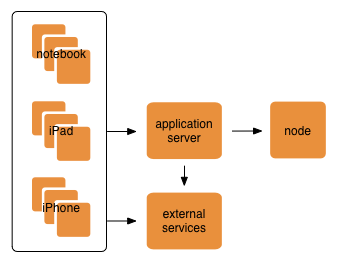
\includegraphics[width=2.5in]{overall-view}}
\end{frame}

\begin{frame}
\frametitle{System Overview --- Into the network}
\centerline{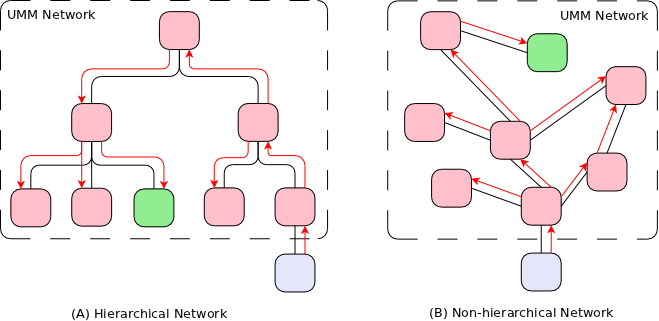
\includegraphics[width=3.5in]{node-hierarchy}}
\end{frame}

\begin{frame}
\frametitle{System Overivew --- Nodes and Routers}
\centerline{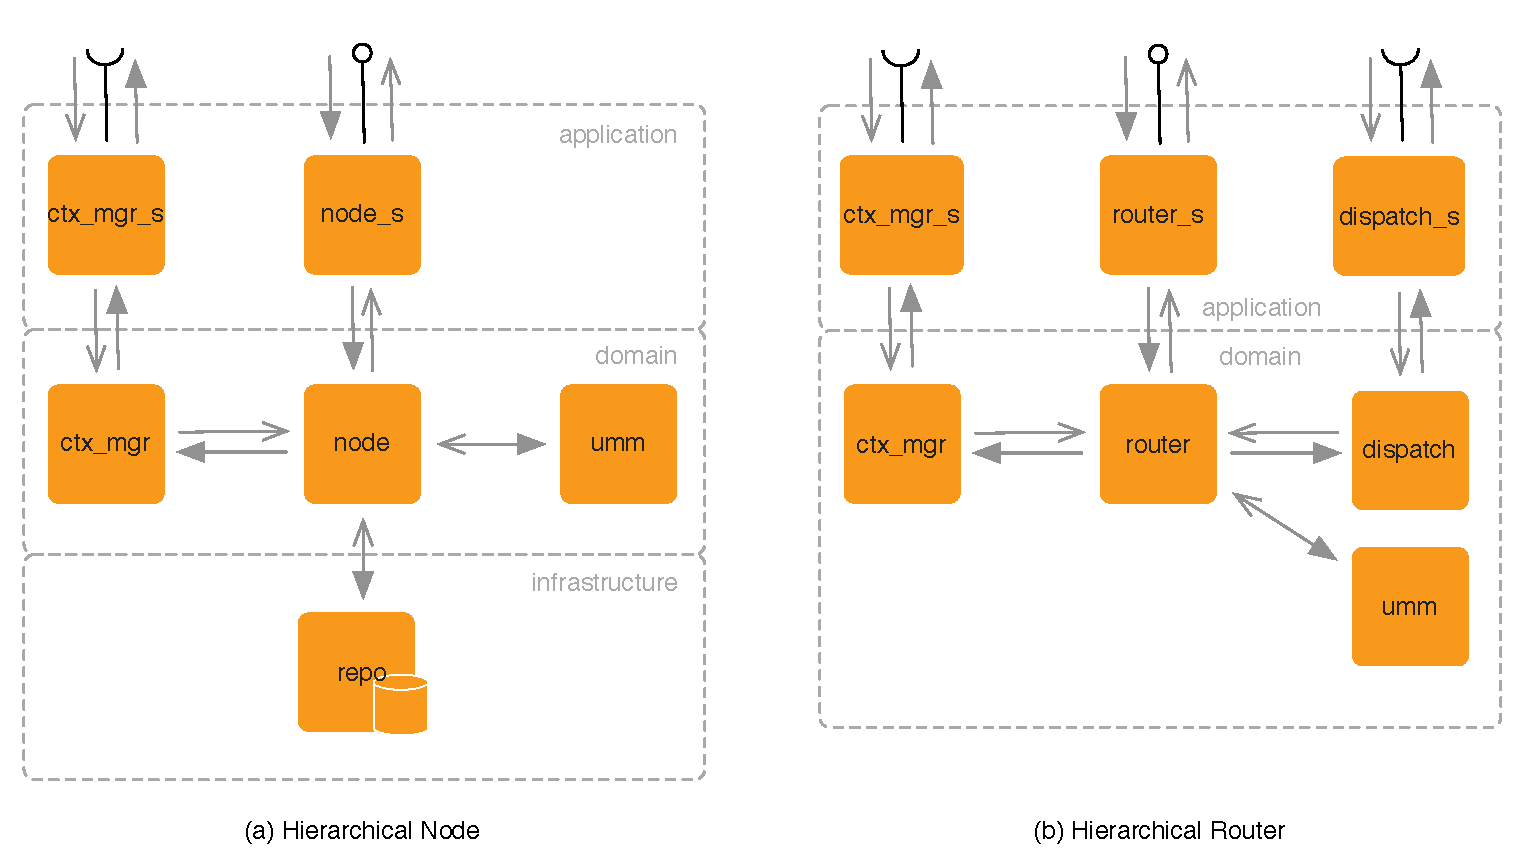
\includegraphics[width=3.5in]{router-node-view}}
\end{frame}

\begin{frame}
\frametitle{Distributed Security Decisions}
\end{frame}

\begin{frame}
\frametitle{Optimal Substructure}
\end{frame}

\begin{frame}
\frametitle{Overlapping Subproblems}
\end{frame}

\begin{frame}
\frametitle{Information Protection}
\end{frame}

\begin{frame}
\frametitle{}
\end{frame}


\end{document}

